\chapter{Конструкторская часть}

\section{Функциональная модель программы}

На рисунке~\ref{img:A0} представлена функциональная модель программы.

\FloatBarrier
\includeimage
{A0} % Имя файла без расширения (файл должен быть расположен в директории inc/img/)
{f} % Обтекание (без обтекания)
{h!} % Положение рисунка (см. figure из пакета float)
{1\textwidth} % Ширина рисунка
{Функциональная модель программы} % Подпись рисунка
\FloatBarrier

\section{Используемые типы и структуры данных}

Для работы программы потребуются следующие структуры данных:

\begin{enumerate}
	\item вершина -- структура, состоящая из координат(трёхмерный вектор), нормали (трёхмерный вектор) и преобразованных координат (четырёхмерный вектор);
	\item матрица размером 4 на 4, состоящая из 16 чисел с плавающей точкой. Требуется для перевода вершин в нужный базис;
	\item камера -- структура, состоящая из позиции (трёхмерный вектор), базиса (3 трёхмерных вектора), фокусного расстояния (число с плавающей точкой) и дальности прорисовки (число с плавающей точкой);
	\item источник света -- структура, состоящая из 2 углов (2 числа с плавающей точкой);
	\item ландшафт -- структура, состоящая из карты высот (двумерный словарь чисел с плавающей точкой) и списка полигонов;
	\item сцена, содержащая в себе все остальные объекты.
\end{enumerate}

\section{Алгоритм, использующий кригинг}

На рисунке~\ref{img:generate} представлена схема алгоритма, использующего кригинг.

\FloatBarrier
\includeimage
{generate} % Имя файла без расширения (файл должен быть расположен в директории inc/img/)
{f} % Обтекание (без обтекания)
{h!} % Положение рисунка (см. figure из пакета float)
{0.45\textwidth} % Ширина рисунка
{Схема алгоритма, использующего кригинг} % Подпись рисунка
\FloatBarrier
 
\section{Построение кадра}

Интенсивность света $I$ вычисляется по закону Ламберта (формула~\ref{eq:lambert}):

\begin{equation}
	\label{eq:lambert}
	I = I_0 \cos{\phi}
\end{equation}

\noindent где $I_0$ -- интенсивность освещения от источника света, а $\phi$ -- угол между нормалью и вектором направления света.

На рисунке~\ref{img:draw} изображена схема алгоритма преобразования координат вершин ландшафта и отсечения перед отрисовкой. На вход подаются матрицы преобразования в систему координат камеры $camera\_matrix$, матрица создания перспективной проекции $frustum\_matrix$, а также фокусное расстояние $focus$.

Матрица перевода в систему координат камеры $camera\_matrix$ получается по формуле~\ref{eq:camera}:

\begin{equation}
	\label{eq:camera}
	camera\_matrix = \begin{pmatrix}
		VX_x & VX_y & VX_z & 0     \\
		VY_x & VY_y & VY_z & 0     \\
		VZ_x & VZ_y & VZ_z & focus \\
		0    & 0    & 0    & 1     \\
	\end{pmatrix}
\end{equation}

\noindent где $VX$, $VY$ и $VZ$ -- векторы базиса камеры, $focus$ - фокусное расстояние камеры.

Матрица создания перспективной проекции $frustum\_matrix$ получается по формуле~\ref{eq:frustum}:

\begin{equation}
	\label{eq:frustum}
	frustum\_matrix = \begin{pmatrix}
		-f & 0      & \frac{width}{2}  & 0     \\
		0      & -f & \frac{height}{2} & 0     \\
		0      & 0      & \frac{v + f}{v} & - \frac{f(v + f)}{v}\\
		0      & 0      & 1                & 0     \\
	\end{pmatrix}
\end{equation}

\noindent где $f$ -- фокусное расстояние камеры, $v$ -- дальность прорисовки, $width$ - ширина экрана, $height$ - высота экрана.

\FloatBarrier
\includeimage
{draw} % Имя файла без расширения (файл должен быть расположен в директории inc/img/)
{f} % Обтекание (без обтекания)
{h!} % Положение рисунка (см. figure из пакета float)
{0.7\textwidth} % Ширина рисунка
{Подготовка полигонов к отрисовке} % Подпись рисунка
\FloatBarrier

%\begin{figure}[h!]
%	\centering
%	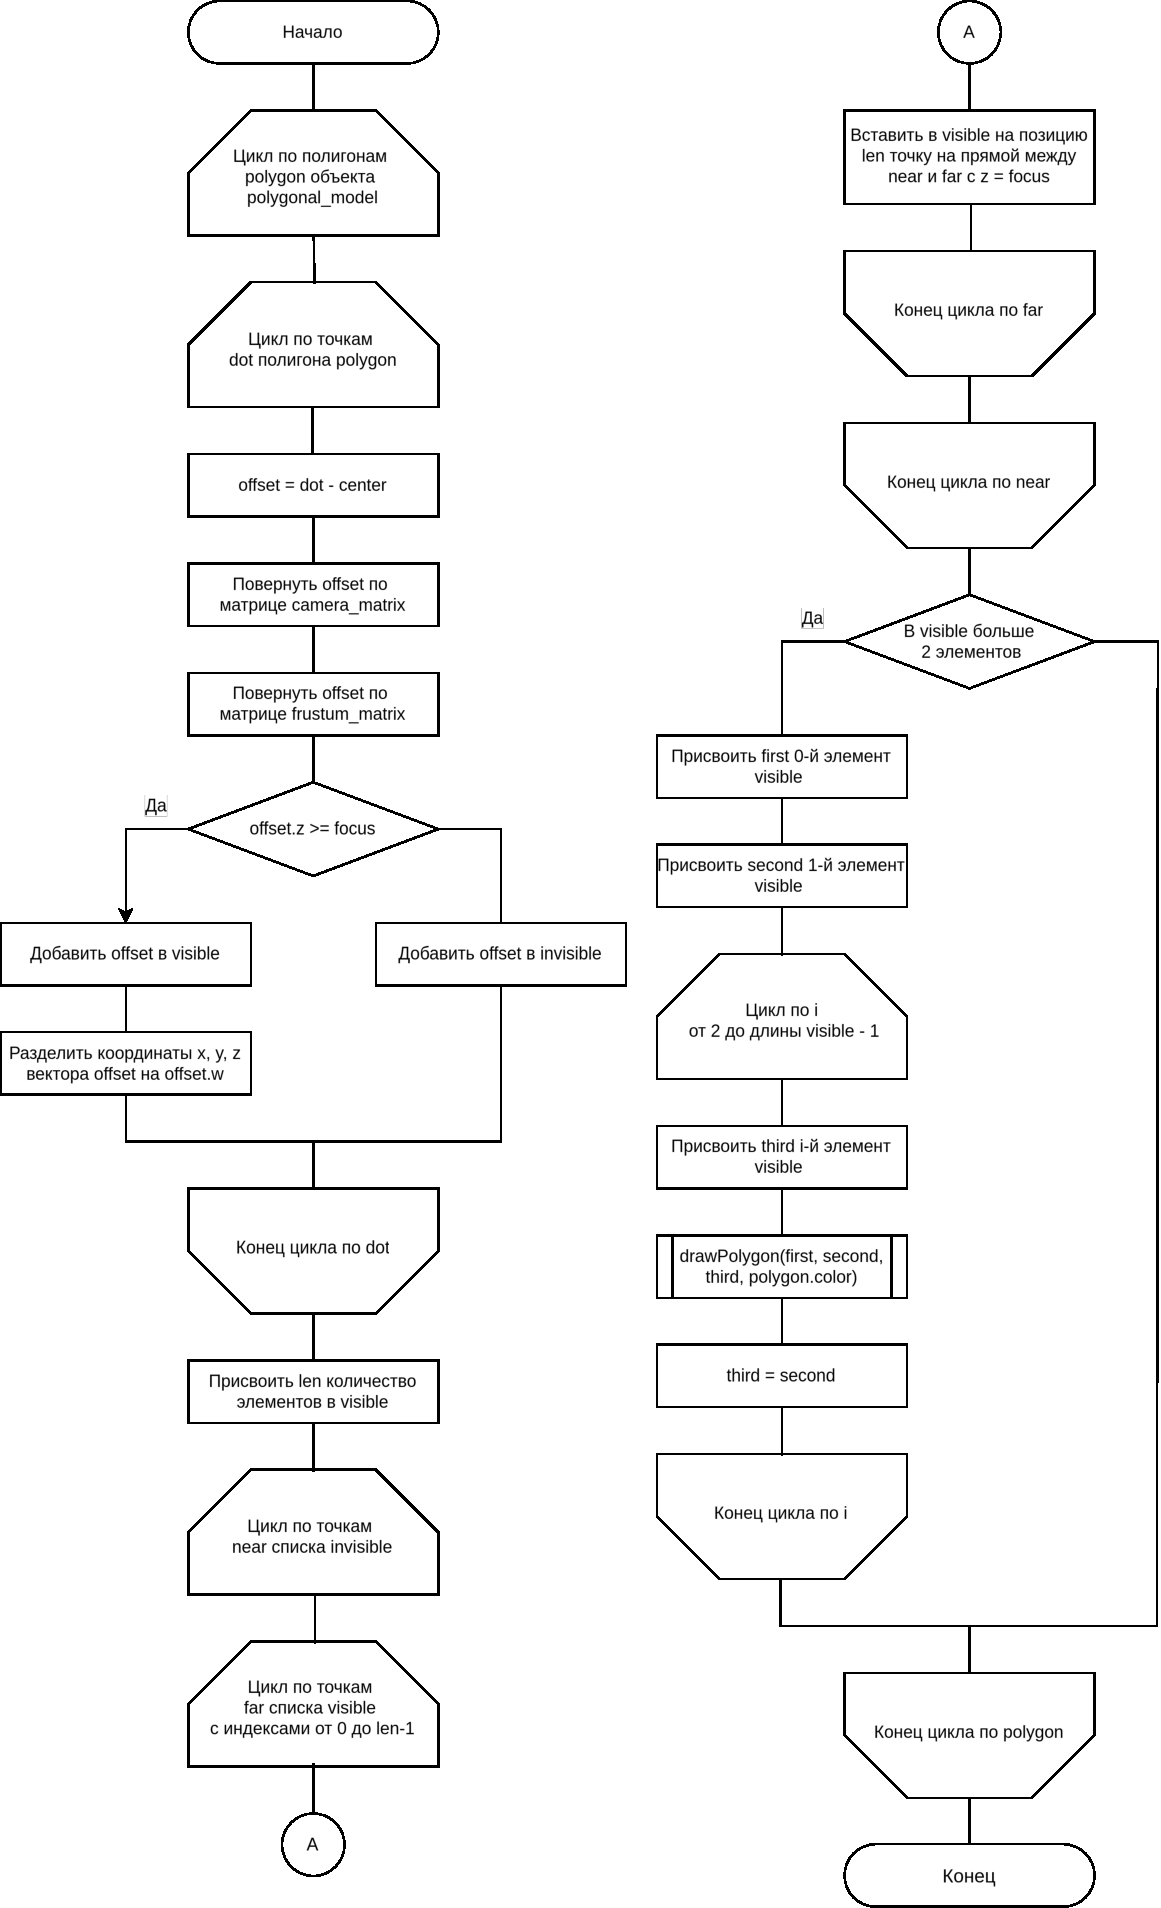
\includegraphics[width=0.6\textwidth]{tex_parts/draw.pdf}
%	\caption{\label{fig:draw}Подготовка данных к отрисовке}
%\end{figure}

На рисунке~\ref{img:z-buffer} изображена схема алгоритма отрисовки полигона. На вход алгоритму передаются 3 преобразованные вершины полигона $A$, $B$, и $C$, интенсивность света в них, цвет полигона $color$, Z-буфер $buffer$.

Координата $z$ произвольной точки D на плоскости ABC вычисляется по формуле~\ref{eq:z}:

\begin{equation}
	\label{eq:z}
	D_z = \alpha A_z + \beta B_z + \gamma C_z
\end{equation}

\noindent где $\alpha$, $\beta$ и $\gamma$ -- барицентрические координаты точки D на плоскости ABC.

Интенсивность света $I$ в точке D вычисляется по формуле~\ref{eq:I}:

\begin{equation}
	\label{eq:I}
	D_I = \alpha A_I + \beta B_I + \gamma C_I
\end{equation}

\FloatBarrier
\includeimage
{z-buffer} % Имя файла без расширения (файл должен быть расположен в директории inc/img/)
{f} % Обтекание (без обтекания)
{h!} % Положение рисунка (см. figure из пакета float)
{0.6\textwidth} % Ширина рисунка
{Отрисовка треугольного полигона с помощью алгоритма, использующего Z-буфер, и закраски Гуро} % Подпись рисунка
\FloatBarrier

\usection{Выводы}

В данном разделе были выбраны структуры данных, а также построены схемы алгоритмов и разработана функциональная схема работы программы.

